\documentclass{llncs} %{IEEEtran}
%\documentclass[14pt]{article}
%\documentclass[conference]{IEEEtran}

\usepackage{multirow,listings,enumerate}
%\usepackage{enumitem}
\usepackage{epsfig,times,subfigure,graphics,amssymb,amsbsy,url,setspace,float,xcolor,tcolorbox,mdframed,listings,sectsty,hyphenat,enumitem}
% \captionsetup[lstlisting]{labelsep=none}

% \sectionfont{\fontsize{15}{15}\selectfont}

\def\inv{\vspace*{-6pt}}
\def\sinv{\vspace*{-3pt}}
\def\smallinv{\vspace*{-3pt}}
\def\smallinh{\hspace*{-3pt}}
\def\smallv{\vspace*{3pt}}
\newcommand{\textbftt}[1]{\textbf{\texttt{#1}}}
\def\tbft[#1]{\textbf{\texttt{#1}}}


%\definecolor{green}{rgb}{0,0.6,0}
%\definecolor{gray}{rgb}{0.5,0.5,0.5}
\definecolor{NavyBlue}{RGB}{15,15,170}
%\usepackage{pythonhighlight}
% See http://ftp.math.purdue.edu/mirrors/ctan.org/macros/latex/contrib/pythonhighlight/pythonhighlight.sty

% pythonhl.sty is a copy of the original pythonhighlight
\usepackage{pythonhl}

% I changed these definitions in pythonhl.sty. Seems to work.
% But I still can't get None to look like a keyword.
% \colorlet{keywordcolour}{black}
% \colorlet{stringcolour}{black}


\definecolor{gray}{gray}{1.0}
\colorlet{commentcolour}{black}
\colorlet{stringcolour}{black}
\colorlet{keywordcolour}{black}
\colorlet{exceptioncolour}{black}
\colorlet{commandcolour}{black}
\colorlet{numpycolour}{black}
\colorlet{literatecolour}{black}
\colorlet{promptcolour}{black}
\colorlet{specmethodcolour}{black}

% % Use this for code snippets
% \lstnewenvironment{python3}[1][]{
% \lstset{
% style=mypython,
% basicstyle=\ttfamily\footnotesize,%\setstretch{.5}, % same as source
% % Put the keywords you want in bold here
% emph={and,break,class,continue,def,yield,del,elif ,else,%
% except,exec,finally,for,from,global,if,import,in,%
% lambda,not,or,pass,None,raise,return,try,while,assert,with},
% % Put the keywords you DO NOT want in bold here
% emph={[2]True, False}
% }
% }


% \lstdefinestyle{pylogPython}{
% language=Python, % Asking for Python 3 doesn't help.
% %basicstyle=\sffamily\small, % print whole listing small. Doesn't seem to matter.
% \sffamily
% % I can't convince it to make None a keyword.
% emph={[2]True, False, None}, % In the original.
% emphstyle=[2]\color{keywordcolour}\bfseries
% emph={[6]assert,None,yield},
% emphstyle={[6]\color{keywordcolour}\bfseries},
% emph={None,and,assert,break,class,continue,def,del,elif,else,%
% except,exec,finally,for,from,global,if,import,in,%
% lambda,not,or,pass,raise,return,try,while,with,yield},
% emphstyle=\color{keywordcolour}\bfseries,
% identifierstyle=\color{RGB}{0, 0, 0},
% morekeywords={None}, 
% otherkeywords={\%, \}, \{, \&, \|, None},
% breaklines=true,
% numbers=left, 
% numberstyle=\small, 
% stepnumber=1, 
% numbersep=5pt, 
% showspaces=false, 
% keepspaces=true, 
% captionpos=b,
% keywordstyle=\color{black}\bfseries, 
% %keywordstyle=\color{NavyBlue},
% commentstyle=\color{green},
% }

% \lstdefinestyle{pylogProlog}{
% language=Prolog, 
% morekeywords={f'}, 
% breaklines=true,
% numbers=left, 
% numberstyle=\small, 
% stepnumber=1, 
% numbersep=5pt, 
% showspaces=false, 
% keepspaces=true, 
% captionpos=b,
% keywordstyle=\color{black}\bf, 
% %keywordstyle=\color{NavyBlue},
% commentstyle=\color{gray}
% }

% \lstdefinestyle{pylog}{% general command to set parameter(s)
% language=Python,
% basicstyle=\small, % print whole listing small
% keywordstyle=\color{black}\bfseries,
% % underlined bold black keywords
% identifierstyle=, % nothing happens
% commentstyle=\color{white}, % white comments
% stringstyle=\ttfamily, % typewriter type for strings
% showstringspaces=false % no special string spaces
% }

% correct bad hyphenation here
\hyphenation{}

%\linespread{0.97}
\usepackage{fancyhdr}
 
\pagestyle{fancy}
\fancyhf{}
\fancyhead[RE,LO]{Pylog}
\fancyhead[LE,RO]{\thepage}
% \fancyhead[RE,LO]{Guides and tutorials}
% \fancyfoot[CE,CO]{\leftmark}

%\input{pythonhighlight.sty}

\begin{document}

%\input{pythonhighlight.sty}

\title{PyLog:}
\author{Russ Abbott \and Jungsoo Lim  \and Jay Patel }
\authorrunning{R. Abbott et al.}
\institute{California State University, Los Angeles, Department of Computer Science \\
          \email{\{jpatel77, jlim34, rabbott\}@calstatela.edu}} 
        
\maketitle
\begin{abstract}
\begin{sloppypar}
Pylog inhabits three programming contexts. 
  \begin{enumerate}[label=\alph*)]
      \item Pylog explores the integration of two distinct programming language paradigms: (i) the modern, general purpose programming paradigm, which includes procedural, object-oriented, and functional programming, and (ii) logic programming, including logic variables (and unification) and depth-first, search. Pylog illustrates how logic programming features can be implemented in and integrated into Python. 
      \item Pylog demonstrates the breadth and broad applicability of Python. Python is both the most widely used language for teaching introductory programming, and it has become widely used for sophisticated programming challenges. 
      \item Pylog exemplifies programming at its best, using Python features in innovative yet clear ways. The overall result is software worth studying. 
 \end{enumerate}
 \end{sloppypar}
\end{abstract}
\section{Introduction}



Prolog, a programming language derived from logic, was developed in the early 1970s. It became very popular during the 1980s as an AI language, especially as part of the Japanese 5th generation project.

Prolog went out of favor because it was difficult to trace the execution of Prolog programs---which made debugging very challenging. But Prolog didn't die and has been making something of a comeback. 
\begin{itemize}
    \item SWI Prolog (free), GNU Prolog (free), and Sictus Prolog (commercial) have kept the Prolog flame burning and have large and active communities of Prolog users.
    \item Sagar \cite{Sagar2019} and Raturi \cite{Raturi2019} both  recommend Prolog for AI programming. 
\end{itemize}
\smallv
Prolog is both one of the syntactically simplest—--you can learn it very quickly--—and at the same time most interesting of all programming language. It is strongly declarative. One first declares facts and rules. (The rules are the Prolog programs.) One then constructs what are called queries, typically with embedded variables, and asks the system to find values for those variables so that the query satisfies the facts and rules. 

Two of Prolog's most distinctive features are logic variables (which support unification) and built-in backtracking search. Prolog was one of the first programming languages with immutable variables. All in all Prolog is seductively elegant and powerful.

Python, of course, is a very well-known and widely used language. It is in first place in the two lists of AI languages mentioned above. Python is one of the easiest programming languages to learn and is used in more introductory programming courses than any other. In addition, Python includes many powerful computational and meta-level capabilities, which facilitate the development of quite sophisticated programs. 
\smallv

Python supports the procedural, object-oriented, and functional programming paradigms. It does not support Prolog's logic programming paradigm. An objective of this work is to show how logic programming can be integrated into standard Python programming.

\section{Related work}

Quite a bit of work has been done in implementing Prolog features in Python, much of it fairly recently. As far as we can tell, none of it is as complete and as fully thought out as Pylog. But nearly all of it makes important contributions. Although, we cannot review the work in detail, following are brief (paraphrased) descriptions from the authors.

\begin{itemize}[label=$~$]

\item Berger (2004) \cite{berger2004}. Pythologic 
\begin{quote}
Python's meta-programming features are used to enable the writing of functions that include Prolog-like features.
\end{quote}

\item Bolz (2007) \cite{Bolz2007} A Prolog Interpreter in Python.  
\begin{quote}
A proof-of-concept implementation of a Prolog interpreter in RPython, a restricted subset of the Python language intended for system programming. Performance compares reasonably well with other embedded Prologs.
\end{quote}

\item Delford (2009) \cite{Delford2009} PyLog. 
\begin{quote}
A proof-of-concept implementation of a Prolog interpreter in RPython.
\end{quote}

\item Frederiksen (2011) \cite{Frederiksen2011} Pike
\begin{quote}
A form of Logic Programming that integrates with Python.
\end{quote}

\item Meyers (2015) \cite{Meyers2015} Prolog in Python. \begin{quote}A hobby project developed over a number of years.\end{quote}

\item Maxime (2016) \cite{Maxime2016} Prology: Logic programming for Python3.
\begin{quote}
A minimal library that brings Logic Programming to Python.
\end{quote}

\item Piumarta (2017) \cite{Piumarta2017} Notes and slides from a course on programming paradigms.

\item Thompson (2017) \cite{Thompson2017} Yield Prolog.
\begin{quote}
Enables the embedding of Prolog-style predicates directly in Python. \end{quote}

\item Santini (2018) \cite{Santini2018} The pattern matching for python you always dreamed of.
\begin{quote}
Pampy is small, reasonably fast, and often makes code more readable.
\end{quote}

\item Cesar (2019) \cite{Cesar2019} Prol: a minimal Prolog interpreter in a few lines of Python. 

\item Kopec (2019) \cite{Kopec2019} Constraint-Satisfaction Problems in Python.  
\begin{quote} Chapter 3 of Kopec (2019) \textit{Classic Computer Science Problems in Python}.
\end{quote}

\item Miljkovic (2019)\cite{Miljkovic2019} 
\begin{quote}
A simple Prolog Interpreter written in a few lines of Python 3.
\end{quote}

\item Niemeyer and Celles (2019) \cite{Niemeyer2019} A python-constraint library.
\begin{quote}
Pure Python solvers for Constraint Satisfaction Problems.
\end{quote}

\item Rocklin (2019) \cite{Rocklin2019} kanren: Logic Programming in Python.
\begin{quote}
Enables the expression of relations and the search for values that satisfy them. (Rocklin is the author of the widely used Python toolz library.)
\end{quote}

\smallv

\end{itemize}

As this short survey illustrates, most of the ideas that provide the foundation for embedding Prolog-like capabilities in Python have been known for a while. What Pylog offers is a more fully developed, more fully explained, and more integrated version.

\input{relatedWork.tex}

\section{From Python to Prolog and back}\label{sec:Pylog}
This section offers a reasonably detained overview of Pylog and how it relates to Prolog. We discuss five small programs, which transition gradually from straight Python to straight Prolog. Listings of these programs are gathered together in section \ref{sec:listings}.
\subsection{Five programs that show the way}
\begin{sloppypar}

Our strategy is to show how a standard Python program can be transformed, step-by-step, into a structurally similar Prolog program. As an example problem, we use the computation of a transversal. 

Given a sequence of sets (in our case lists), a transversal is a non-repeating sequence of elements with the property that the \textit{n\textsuperscript{th}} element of the traversal belongs to the \textit{n\textsuperscript{th}} list/set in the sequence. For example, the sets (actually lists\footnote{From here on, we refer informally to the lists in our example as \textit{sets}.}) [[1, 2, 3], [2, 4], [1]] have three transversals: [2, 4, 1], [3, 2, 1], and [3, 4, 1]. We use the transversal problem because it lends itself to depth-first search, the default Prolog control structure.\footnote{We use traditional, i.e., naive, depth-first search. Most modern Prologs include a constraint processing package such as CLP(FD)\cite{Triska2016}, which makes search much more efficient.

Instead of scanning the sets in the order given, one can select the next set to scan based on how constrained the sets are. In the case of [[1, 2, 3], [2, 4], [1]], the third set would be scanned first, with 1 selected as its representative in any transversal. 

Another efficiency measure involves propagating constraints. Suppose our example sets are scanned from left to right. If 1 is selected from the first set, that choice would be propagated forward, eliminating 1 from the final set. Since the final set would then have no choices left, one can conclude that selecting 1 from the first set does not lead to a solution. 

Application of such constraint rules eliminate much of the backtracking inherent in naive depth-first search. Powerful as they are,we do not consider such constraint techniques.}

We will discuss five functions for finding transversals. In the course of discussing these programs we will introduce various Pylog features. Here is a road-map for the programs to be discussed and the Pylog features they illustrate. The first four are written in Python. The final one is in standard Prolog. 
\begin{enumerate}
\item \textittt{transversal\_dfs\_first} is a standard Python program that performs a depth-first search. It stops and returns the first transversal it finds. It contains no Pylog features, but it defines a structure the other programs follow. 
\smallv
 
\item \textittt{transversal\_dfs\_all}. In contrast to \textittt{transversal\_dfs\_first}, the program \textittt{transversal\_dfs\_all} finds and returns \textit{all} transversals. The most common strategy, and the one \textittt{transversal\_dfs\_all} uses, is to gather all transversals into a package, which is returned at the end.
\smallv

\item \textittt{transversal\_dfs\_yield} solves the problem of finding all transversals, but it returns them one at a time. \textittt{transversal\_dfs\_all} does this through the use of the Python generator structure, i.e., the \textbftt{\textbf{yield}} statement. This moves us an important step toward a Prolog-like control structure.
\smallv
    
\item \textittt{transversal\_dfs\_yield\_lv} introduces logic variables, one of the most important features of Prolog.  

\item \textittt{transversal\_prolog} is a straight Prolog program. It is operationally identical to \textittt{transversal\_dfs\_yield\_lv}, but syntactically very different. 
\end{enumerate}

Now we will look at these programs in a bit more detail. The first three Python programs have similar signatures. 

\begin{python}
def transversal_python_1_2_3(sets: List[List[int]], 
                             partial_transversal: List[int])
                             -> <some return type>: 
\end{python}
(The return types differ from one program to an other.)

Both the fourth Python program and the Prolog program have a third parameter. Their return type, if any, is not meaningful for our purposes. Each transversal, when found, is returned through the third parameter---as one does in Prolog.

\begin{python}
def transversal_python_4(sets: List[List[int]], 
                         partial_transversal: List[int],
                         Complete_Transversal: Var)
\end{python}

\begin{python}
    transversal_prolog(+Sets, 
                       +Partial_Transversal, 
                       -Complete_Transversal)
\end{python}

The signatures have the following in common. 
\begin{enumerate}
\item The first argument lists the sets for which a transversal is desired. Initially this is the full list of sets. The programs recursively step through the list, selecting an element from each. At each recursive call, the first argument lists the remaining sets. 

\item The second argument is a partial transversal consisting of elements selected from sets that have already been scanned. Initially, this argument is the empty list.

\item The third parameter and the return type.
\begin{enumerate}
\item The first two programs have no third argument. They return a single transversal, a set of transversals, or \textbftt{None} through the normal \textbftt{return} mechanism.

\item The final Python function and the Prolog predicate both have a third parameter. Neither returns a value through a normal \textbftt{return} mechanism. In both, the third argument is initially an uninstantiated logic variable, which will be unified with a transversal that is being returned.
\end{enumerate}
\end{enumerate}
The following discusses the functions in more detail.
\begin{itemize}[label=$\bullet$]
\item \textittt{transversal\_dfs\_first}. The first Python program uses standard depth-first recursion to find a single transversal. As listing \ref{lis:dfsfirst} shows, when we reach the end of the list of sets, we are done. At that point we return  \textit{partial\_transversal}, which at that point is known to be a complete transversal. The return type is \textittt{Optional[List[int]]}, i.e., either a list of \textittt{int}s, or \textbftt{None} for the case in which no transversal is found. The latter situation occurs when, after considering all elements of set (line 10), we have not found a complete transversal. The program then runs off the end of the \textbftt{else} clause, returning \textbftt{None}.

It may be instructive to look at listing \ref{lis:dfsfirsttrace}, created by the print statement in the first line.\footnote{All the programs in this section produce a log. This is the only log included in this paper.} It shows the value of the parameters at the start of each execution of the function. When \textittt{sets} is the empty list (line 7), we have found a transversal. 
\smallv
    
On the other hand, when the function reaches a dead-end, it backtracks to the most recent point at which it selected a tentative transversal element. For example, the first three lines show that we have selected \textittt{[1, 2]} as the \textittt{partial\_transversal} and must now select an element of \textittt{[1]}, the remaining set. Since \textittt{1} is already in the \textittt{partial\_transversal}, it can't be selected to represent the final set. So we (blindly, as is the case with naive depth-first search) backtrack to the selection from the second set. We had initially selected \textittt{2}. Line 4 shows that we now select \textittt{4}. Of course that doesn't help. Having exhausted all elements of the second set, we backtrack all the way to our selection from the first set.
\smallv
    
Line 5 of the log shows that we have now selected \textittt{2} from the first set and are about to make a selection from the second set. The log does not show that we considered selecting \textittt{2} from the second set but that since it was already in the \textittt{partial\_transversal}, we moved on to selecting \textittt{4} from the second set. We are then able to select \textittt{1} from the final set.
\smallv
    
Even though this is a simple Python depth-first search, it incorporates (what appears to be) backtracking, one of the mainstays of Prolog. What implements the backtracking? There is no backtracking. We simply have recursively nested \textbftt{for} loops, which produce a backtracking effect. 
\smallv

Prolog, uses the term \textit{choicepoint} for places in the program at which (a) multiple choices are possible and (b) one wants to try them all if necessary. Pylog implements choicepoints by means of such nested \textbf{for} loops and related mechanisms.

\item \textittt{transversal\_dfs\_all}. The second Python program finds and returns \textit{all} transversals. It has the same structure as \textittt{transversal\_dfs\_first} except that instead of returning a single transversal, each transversal is added to \textittt{all\_transversals} (line 12). The entire list is returned when the program terminates. 

~ Note that \textittt{transversal\_dfs\_first} returns \textbftt{None} if no transversal is found whereas \textittt{transversal\_dfs\_all} returns an empty list. Hence the return type of \textittt{transversal\_dfs\_all} is \textittt{List[List[int]]} rather than \textittt{Optional[List[int]]}. 
\smallv

\item  \textittt{transversal\_yield}. 
The third Python program, although quite similar to the first, takes a significant step toward mimicking Prolog. Whereas \textittt{transversal\_dfs\_first} \textbftt{return}s the first transversal it finds, \textittt{transversal\_yield} \textbftt{yield}s \textit{all} the transversals it finds---but one at a time.  Instead of looking for a single transversal on lines 12 and 13 with:
\begin{python}
complete_transversal =  \ 
  transversal_dfs_first(ss, partial_transversal + [element])
\end{python}
and then \textbftt{return}ing those that are not \textbftt{None}, \textittt{transversal\_yield} uses  (line 12) \textbftt{yield} \textbftt{from} to search for and \textbftt{yield} \textit{all} transversals---but one at a time.
\begin{python}
yield from transversal_yield(ss, partial_transversal + [element])
\end{python}

\item  \textittt{transversal\_yield\_lv}. The fourth Python program moves toward Prolog along a second dimension---the use of logic variables.
\smallv

One of Prolog's defining features is its logic variables. A logic variable is similar to a variable in mathematics. It may or may not have a value, and once it gets a value, its value never changes, i.e., logic variables are immutable.
\smallv

The primary operation on logic variables is known as \textit{unification}. When a logic variable is \textit{unified} with what is known as a \textit{ground term}, e.g., a number, a string, etc., it acquires that term as its value. For example, if \textittt{X} is a logic variable,\footnote{A note about identifiers. The Python convention is to use only lower case letters in identifiers other than class names. The Prolog convention is that the first letter of an identifier determines whether it's a constant term or a variable. Variables begin with upper case letters. 
\smallv
    
In the first three programs we have used strictly lower case letters in identifiers. In \texttt{transversal\_yield\_lv}, and of course in the Prolog program to follow, we use upper case letters to begin identifiers that refer to Prolog or Prolog-like variables. Thus the \textittt{X} and  \textittt{Y} in this discussion begin with upper case letters. In \textittt{transversal\_yield\_lv}, the identifiers \textittt{Partial\_Transversal} and \textittt{Complete\_Transversal} begin with upper case letters. Even though they are Python variables, they are used as Pylog logic variables.} then after \textittt{unify(3, X)},\footnote{or \textittt{unify(X, 3)}, the order of the arguments is not relevant} \textittt{X} has the value \textittt{3}. 
Like mathematical variables, logic variables may be set equal to each other---even if neither has a value. So if \textittt{X} and \textittt{Y} are two logic variables, then after \textittt{unify(X, Y)} whatever value either eventually gets will be considered the value of the other. For example, after
\begin{python}
(A, B, C, D, E) = (Var(), Var(), Var(), Var(), 'def')
for _ in unify(A, B):
  for _ in unify(D, C):
    for _ in unify(A, C):
      for _ in unify(E, D):
\end{python}
\textittt{A}, \textittt{B}, \textittt{C}, \textittt{D}, and \textittt{E} all have the value \textittt{'def'}.
\smallv

Two convenience methods\footnote{
$\bullet$ \textittt{n\_Vars} takes an integer argument and generates that many \textittt{Var} objects.\newline
$\bullet$ \textittt{unify\_pairs} takes a list of pairs (as tuples) and unifies the two elements of each pair.
} 
make it possible to write the preceding more concisely.
\begin{python}
(A, B, C, D, E) = (*n_Vars(4), 'def')
for _ in unify_pairs([(A, B), (D, C), (A, C), (E, D)]):
\end{python}
\smallv
Since \textit{unify} and \textit{unify\_pairs} are both generators, they must be called from something like a \textbf{for} loop as shown---rather than as  standard function calls.
\smallv

Here are a few additional important considerations.
\begin{itemize}[label=$\circ$]
\item  \textit{transversal\_yield\_lv} has a third parameter, \textit{Complete\_Transversal}, which is declared as a \textit{Var}, i.e., a logic variable. When \textit{transversal\_yield\_lv} is called initially, \textit{Complete\_Transversal} is uninstantiated. If \textit{Sets} is empty, we perform \textit{unify(Partial\_Transversal, Complete\_Transversal)}, which gives \textit{Complete\_Transversal} the same value as \textit{Partial\_Transversal}. This is typical of how Prolog programs return values: unify an argument with the value to be returned.
\item The \textbftt{else} clause (line 8) defines \textit{Element} to be a \textit{Var}. The line 
\begin{python}
    for _ in member(Element, S):
\end{python}
unifies \textit{Element} with a member of \textit{S} each time around the loop. 
\smallv

\item The syntax of the \textbftt{for} iterator/generator loop is worth a remark. The function \textit{member} is written to perform its own \textit{unify} operation and then to perform a \textit{yield}. This makes it suitable for use in a \textbf{for} iterator/generator loop as shown. 
\smallv

The \textbftt{for} loop itself does not produce a value in the normal way. (Note the underscore.) Instead, after \textit{member} unifies its first argument with an element of its second, it \texttt{\textbf{yield}}s to indicate that the unification is complete. For example, 
\begin{python}
Element = Var()
for _ in member(Element, S):
  print(Element)
\end{python}
prints the elements of \textit{S}.
\smallv

\item In earlier functions (line 10) we had written 
\begin{python}
if element not in partial_transversal:
\end{python}
In \texttt{transversal\_yield\_lv} we write (line 12)
\begin{python}
for _ in fails(member)(Element, Partial_Transversal):
\end{python}
The Pylog \textit{fails} function does the same job as \textit{\textbackslash+}, i.e., negation, in Prolog. \textit{fails} takes another function as an argument---much like a Python decorator ---and returns a function that succeeds or fails when its argument function fails or succeeds. Thus, although it's not boolean,
\begin{python}
for _ in fails(member)(Element, Partial_Transversal):
\end{python} 
is approximately equivalent to
\begin{python}
if element not in partial_transversal:
\end{python}
\smallv

For double negation, i.e., Prolog's \texttt{\textbackslash+\textbackslash+}, Pylog offers \textit{would\_succeed} rather than a pair of nested \textit{fails}.
\begin{python}
for _ in would_succeed(member)(Element, S):
\end{python} 
succeeds if and only if
\begin{python}
for _ in member(Element, S):
\end{python} 
would succeed. The only (but very important) difference is that, as in  Prolog's double negation, \textit{would\_succeed} does not unify any variables.
\smallv

\item Consider line 13 of the listing. It uses Python's \textbftt{yield from} construct. 

\begin{python}
  yield from <something>
\end{python}
can be considered shorthand for 
\begin{python}
for X in <something>:
  yield X
\end{python}
As before, \textittt{X} may be an underscore, in which case nothing is returned, and the \textbftt{yield} statement is simply \textbftt{yield} with no argument.
% \smallv
% 
% \footnote{
% \begin{quote}
% It's unfortunate that Python doesn't offer a bit more syntactic flexibility. The construct:
% \begin{python}
% for _ in generator:
% \end{python} 
% is really setting a context for what follows. Pylog offers the following alternatives.
% \begin{python}
% with generator_function(args) as generator:
%     while generator.has_more():
%         ...
% \end{python} 
% and 
% \begin{python}
% generator = generator_function(args)
%     while generator.has_more():
%         ...
% \end{python} 
% But neither of these seems better.
% \end{quote}
% }
\smallv

Consider how \textbftt{yield} \textbftt{from} is used in this program. It performs four functions.
\begin{enumerate}
\item It calls the remaining program to be executed. In this case, it's a recursive call, but that need not be the case.
\item It passes to the called function values from previously executed code. 
\item It also passes on an uninstantiated variables---the third argument---which the remainder of the program will (presumably) instantiate.
\item Since it functions as a \textbftt{yield}, it returns what will be the newly instantiated argument back up the  \textbftt{yield} chain.
\end{enumerate}
\smallv

We can put this into a Prolog context. Consider a standard Prolog clause.
\smallv

\begin{python}
    head(<args>) :-
        term_1(<args_1>),
        term_2(<args_2>), 
        ...
        term_n(<args_n>).
\end{python}
The relationship between a clause head and its body as well as that between each term and the rest of the body is exactly a \textbftt{yield from} relationship. 
\smallv
\end{itemize}

\item \textittt{transversal\_prolog}. The final program is straight Prolog. Inspection of the listing will show that \textit{transversal\_prolog} and \textit{transversal\_yield\_lv} are the same program expressed in different languages.

\end{itemize}
\end{sloppypar}

% \subsection{Cryptarithmetic Problem}
% Cryptarithm, mathematical recreation in which the goal is to decipher an arithmetic problem in which letters have been substituted for numerical digits.
% The term crypt-arithmetic was introduced in 1931, when a multiplication problem appeared in the Belgian journal Sphinx [Fig. 1]:
% \begin{figure}
% \centerline{
% 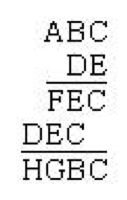
\includegraphics[width=0.15\textwidth]{fig/fig_crypt_1.png}}
% \caption{Cryptarithmetic Multiplication Problem}
% \label{fig:crypt_multi}
% \end{figure}

% Cryptarithm now denotes mathematical problems usually calling for addition, subtraction, multiplication, or division and replacement of the digits by letters of the alphabet or some other symbols.\footnote{\textit{Cryptarithm} is defined in \cite{BritannicaCrypt}.}

% The problem discussed here involves a simple addition of two terms consisting of characters resulting in a sum term. The goal is to map each character to a digit such that the summation of two numeric terms matches the character mapping of the sum term.
% Here are some of the constraints:
% \begin{itemize}
% \item Leading character for each term cannot be mapped to 0
% \item There should be no more than 10 distinct characters. For example, $abcde+efghi=ijklm$ has no solutions (there are 12 distinct characters)
% \item The summation should be the longest word. For example, $ab+cde=fg$ has no solutions ($cde$ is longer than $fg$)
% \item The summation cannot be too long. For example, $ab+cd=efgh$ has no solutions ($ab$ and $cd$ range from 10 to 99, so the summation cannot be more than 198).\footnote{These are mentioned as tips in \cite{CryptPuzzleSolver}.}
% \end{itemize}

% For example,
% \begin{figure}
% \centerline{
% 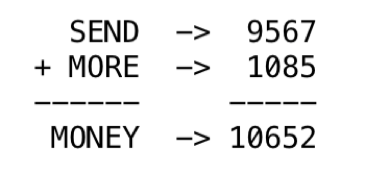
\includegraphics[width=0.5\textwidth]{fig/fig_crypt_2.png}}
% \caption{Cryptarithmetic Summation Problem}
% \label{fig:crypt_sum}
% \end{figure}

% Due to the nature of the problem, there might exist more than one solution to it. The goal is to find all such solutions.

% One way is to try to fill the columns from right to left, by assigning (unifying) valid digits to characters as we move to the left. In the beginning, the digit pool will have all 10 digits to choose from. Once we assign a digit to a character, we remove it from the digit pool. Doing this keeps us from picking the already assigned digit again for a different character (eliminating possibilities). When we reach the leftmost column and successfully assign a digit to the final character, we get the one possible solution to the problem.

% At any point during assignment (unification), if we come across an invalid choice, we will skip to the next available choice until we exhaust all the choices from the digit pool. In which case, we backtrack to the previous level, make a different choice and continue from there. This mimics the depth-first-search which is a core functionality of Prolog. To achieve the same in Python, we will make use of PyLog.

% First, we will set up the problem into a proper representation. 
% \begin{enumerate}
% \item Create a dictionary of a character to an uninstantiated PyValue for all unique characters
% \item Create 4 lists of PyValues for carries, term1, term2 and sum
% \item Length of each list would be the length of the sum term plus 1
% \item Pad all three terms with PyValue(0) and fill the remaining with uninstantiated PyValue instance from the dictionary
% \item Fill the carry list with unique uninstantiated PyValues
% \item Create a list leading\_digits that maintains all the PyValue instances that are at the beginning of any term. We use this to avoid unifying digit 0 to any of these PyValue.
% \end{enumerate}

% Here is how it will look like:
% \begin{figure}
% \centerline{
% 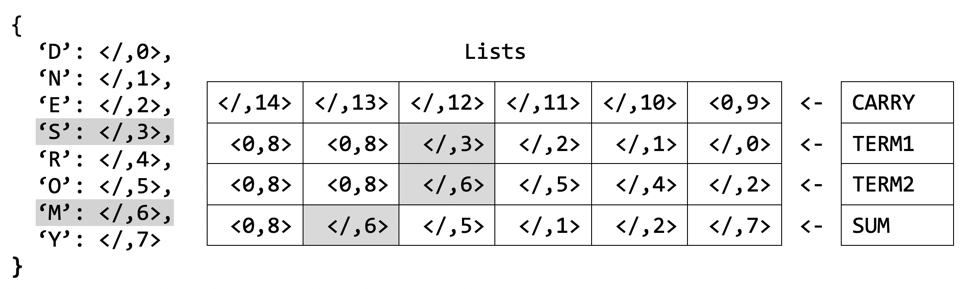
\includegraphics[width=\textwidth]{fig/fig_crypt_3.png}}
% \caption{Graphical Representation of the problem setup}
% \label{fig:crypt_setup}
% \end{figure}
 
% Here, each \pyth{<value, obj_id>} represents a PyValue object. As discussed above, each list contains a PyValue object. It can be seen that a character is represented by the same PyValue object across all 3 arrays (i.e. Term1, Term2 and Sum array). For example, ‘E’ appears in all 3 terms, and is represented by the same object \pyth{</,2>} in all 3 lists.

% Some of the fields are grayed out. These are the leading characters, and therefore cannot be assigned to a digit 0. We keep track of this by looking at leading\_digits list.

% Here is a code that achieves the above setup:

% \begin{python3}
% def set_up_puzzle(t1: str, t2: str, sum: str, _Z: PyValue) -> \
%                   Optional[Tuple[List[PyValue], List[PyValue], List[PyValue], List[PyValue], List[PyValue]]]:
%   """
%   Convert the initial string representation to (uninstantiated) PyValues.
%   t1 and t2 are the numbers to be added. sum is the sum.
%   _Z is PyValue(0). It will be replaced by leading blanks.
%   """
%   Var_Letters = sorted(list(set(t1 + t2 + sum)))
%   if len(Var_Letters) > 10:
%     print(f'Too many variables: {Var_Letters}')
%     return
%   Vars_Dict = {V: PyValue() for V in Var_Letters}
%   length = len(sum) + 1
%   T1 = (length - len(t1)) * [_Z] + letters_to_vars(t1, Vars_Dict)
%   T2 = (length - len(t2)) * [_Z] + letters_to_vars(t2, Vars_Dict)
%   Sum = (length - len(sum)) * [_Z] + letters_to_vars(sum, Vars_Dict)
%   # Leading_Digits are the variables that should not be assigned 0.
%   Leading_Digits = letters_to_vars({t1[0], t2[0], sum[0]}, Vars_Dict)
%   Carries = [PyValue() for _ in range(length - 1)] + [PyValue(0)]
%   return (Carries, T1, T2, Sum, Leading_Digits)
% \end{python3}
% \begin{lstlisting} [caption={cryptarithmetic\_set\_up\_puzzle},  label={lis:cryptarithmetic}]
% \end{lstlisting}

% Now that we have a setup, we can start solving the puzzle. To solve the puzzle, all we need is the parameters Carries, T1, T2, Sum, and Leading\_Digits created above. If it finds a valid solution, it yields at that point. We capture this yield, which acts like a halt in the execution of a function and prints out the state of all the PyValue objects to the console. This is one solution to the puzzle. We can iterate through this generator function until exhaustion to find out all possible solutions to the puzzle. Here is a code that iterates through the solve() generator function.

% \begin{python3}
% def solve_crypto(t1: str, t2: str, sum: str):
%   _Z = PyValue(0)
%   (Carries, T1, T2, Sum, Leading_Digits) = set_up_puzzle(t1, t2, sum, _Z)
%   want_more = None
%   Blank = PyValue(' ')
%   for _ in solve(Carries, T1, T2, Sum, Leading_Digits):
%     # We have a solution.
%     # Replace the leading _Z zeros with blanks and convert each number to a string.
%     # We can discard T1[0], T2[0], and Sum[0] because we know they will be 0.
%     (t1_out, t2_out, tot_out) = (solution_to_string(T, _Z, Blank) for T in [T1[1:], T2[1:], Sum[1:]])
%     print()
%     print(f'  {t1}  -> {t1_out}')
%     print(f'+ {t2}  -> {t2_out}')
%     print(f'{"-" * (len(sum)+1)}     {"-" * len(sum)}')
%     print(f' {sum}  -> {tot_out}')
%     ans = input('\nLook for more solutions? (y/n) > ').lower( )
%     want_more = ans[0] if len(ans) > 0 else 'n'
%     if want_more != 'y':
%       break
%   if want_more == 'y':
%     print('No more solutions.')

% \end{python3}
% \begin{lstlisting} [caption={cryptarithmetic\_solve\_crypto},  label={}]
% \end{lstlisting}

% Let’s talk about how the solve() function solves the puzzle. It starts filling columns from right to left. fill\_column() takes the list of PyValue objects of a column and list of all the available digits to choose from as input. Once it completes filling a column, it yields back the remaining digits in the form of a list. These remaining digits are then passed on to the next fill\_column() call to fill the next column. Once the last column is filled successfully, it halts the execution of solve() by yield statement.

% fill\_column() works in a recursive manner. It iterates through all the available digits from the pool and assigns (unifies) the digit to the first PyValue from the input list, and recursively calls itself for the remaining PyValues and digit pool. Once all the PyValues are assigned (i.e. PVs == False), it performs the validation of the current choices. It sums up the values of terms’ PyValues along with the carry at the current index, finds the mod of 10, and matches it to the expected sum digit to the current index. If this holds, meaning current choices are correct for the column, it assigns (unifies) the remaining carry value to the next index’s carry. These operations are taken care of by a method complete\_column().

% Once the last column is filled, to check if the solution is valid or not, it performs the last check where it ensures there is no leftover carry stored in the first object of the carry list.

% It very crucial that, while unifying any PyValue with a digit, we need to first ensure that it is uninstantiated i.e. it has not been unified with any digit yet. A PyValue object has a method is\_instantiated() which returns a Boolean that tells if the object is already unified or not.

% One more important point to take note is the constraint that any leading character cannot be unified with a digit 0. We ensure this by putting the check \pyth{if not (digits_in[i] == 0 and PV in Leading_Digits)} while choosing a digit for the current PyValue instance.

% The following is the code that achieves the above solution.

% \begin{python3}
% def solve(Carries: List[PyValue],
%           Term1: List[PyValue],
%           Term2: List[PyValue],
%           Sum: List[PyValue],
%           Leading_Digits: List[PyValue]):
%   """
%   Solve the problem.
%   The two embedded functions below refer to the lists in solve's params.
%   The lists never change, but their elements are unified with values.
%   No point is copying the lists repeatedly. So embed the functions that refer to them.
%   """

%   def fill_column(PVs: List[PyValue], index: int, digits_in: List[int]):
%     """
%     PVs are the digits in the current column to be added together, one from each term.
%     digits-in are the digits that have not yet been assigned to a Var.
%     Find digits in digits_in that make the column add up properly.
%     Return (through yield) the digits that are not yet used after the new assignments.
%     We do this recursively on PVs--even though we are currently assuming only two terms.
%     """
%     if not PVs:
%       # We have instantiated the digits to be added.
%       # Instantiate Sum_Dig (if possible) and Carries[index - 1] to the total.
%       # Completing the column is a bit more work than it might seem.
%       (carry_in, digit_1, digit_2) = (D.get_py_value( ) for D in [Carries[index], Term1[index], Term2[index]])
%       total = sum([carry_in, digit_1, digit_2])
%       (carry_out, sum_dig) = divmod(total, 10)
%       yield from complete_column(carry_out, Carries[index-1], sum_dig, Sum[index], digits_in, Leading_Digits)

%     else:
%       # Get head and tail of PVs.
%       [PV, *PVs] = PVs
%       # If PV already has a value, nothing to do. Go on to the remaining PVs.
%       if PV.is_instantiated( ):
%         yield from fill_column(PVs, index, digits_in)
%       else:
%         # Give PV one of the available digits. Through "backup" all digits will be tried.
%         for i in range(len(digits_in)):
%           if not (digits_in[i] == 0 and PV in Leading_Digits):
%             for _ in unify(PV, digits_in[i]):
%               yield from fill_column(PVs, index, digits_in[:i] + digits_in[i + 1:])

%   def solve_aux(index: int, digits_in: List[int]):
%     """ Traditional addition: work from right to left. """
%     # When we reach 0, we're done.
%     if index == 0:
%       # Can't allow a carry to this position.
%       if Carries[0].get_py_value() == 0:
%         yield
%       else:
%         # If we reach index == 0 but have a carry into the last column, fail.
%         # Won't have such a carry with only two terms. But it might happen with many terms,.
%         return
%     else:
%       for digits_out in fill_column([Term1[index], Term2[index]], index, digits_in):
%           yield from solve_aux(index-1, digits_out)
    
%   yield from solve_aux(len(Carries)-1, list(range(10)))


% def complete_column(carry_out: int, Carry_Out_Dig: PyValue,
%                     sum_dig: int, Sum_Dig: PyValue,
%                     digits_in: List[int], Leading_Digits):
%   """
%   If Sum_Dig (the variable representing the digit in the sum for this column) is not yet instantiated,
%   instantiate it to sum_dig  (if that digit is available). If Sum_Dig is already instantiated, ensure
%   it is consistent with the sum_dig. Instantiate Carry_Out_Dig to carry_out.
%   """
%   # Is Sum_Dig uninstantiated? If so, instantiate it to sum_digit if possible.
%   # Then instantiate Carry_Out_Dig, and return (yield) digits_in with sum_digit removed.
%   if not Sum_Dig.is_instantiated():
%     if sum_dig not in digits_in:
%       # sum_dig is not available in digits_in. Fail, i.e., return instead of yield.
%       return

%     # sum_dig is available in digits_in. Give it to Sum_Dig as long as this does not give
%     # 0 to one of the leading digits.
%     if not (sum_dig == 0 and Sum_Dig in Leading_Digits):
%       for _ in unify_pairs([(Carry_Out_Dig, carry_out), (Sum_Dig, sum_dig)]):
%         # Remove sum_digit from digits_in
%         i = digits_in.index(sum_dig)
%         yield digits_in[:i] + digits_in[i + 1:]

%   # If Sum_Dig is instantiated, is it equal to sum_digit?
%   # If so, instantiate Carry_Out_Dig and return the current digits_in.
%   elif sum_dig == Sum_Dig.get_py_value( ):
%     for _ in unify(Carry_Out_Dig, carry_out):
%       yield digits_in
% \end{python3}
% \begin{lstlisting} [caption={cryptarithmetic\_solve},  label={}]
% \end{lstlisting}

\section{Zebra Problem}\label{subsec:zebra}
The Zebra Puzzle, also known as the Einstein's Riddle, is a well known logic puzzle. 
\smallv

There are five houses in a row. Each is occupied by a family of unique nationality. Each has a unique favorite smoke, a unique pet, a unique favorite drink, and a unique color. Fourteen clues, see below, provide additional constraints. With the given information, determine: \textit{Who has a zebra and who drinks water?}
\smallv

One can easily write Prolog programs to solve this and similar puzzles.
\begin{itemize}[label=$\bullet$]
\item We represent a house as a Prolog term with five fields:
\smallv

\begin{python}
    house(<nationality>, <smoke>, <pet>, <drink>, <color>)
\end{python}
\item Our "world" will be a list of 5 houses, with all fields initially uninstantiated.  
\smallv

\item The clues can be written as more-or-less direct translations of the English.
\end{itemize}

\begin{python}
zebra_problem(Houses) :-
    Houses = [house(_,_,_,_,_),house(_,_,_,_,_),house(_,_,_,_,_),
              house(_,_,_,_,_),house(_,_,_,_,_)],
    % 1. The English live in the red house.
    member(house(english,_,_,_,red), Houses),
    % 2. The Spanish have a dog.
    member(house(spanish,_,dog,_,_), Houses),
    % 3. They drink coffee in the green house.
    member(house(_,_,_,coffee,green), Houses),
    % 4. The Ukrainians drink tea.
    member(house(ukranians,_,_,tea,_), Houses),
    % 5. The green house is immediately to the right of the white house.
    nextto(house(_,_,_,_,white), house(_,_,_,_,green), Houses),
    % 6. The Old Gold smokers have snails.
    member(house(_,old_gold,snails,_,_), Houses),
    % 7. They smoke Kool in the yellow house.
    member(house(_,kool,_,_,yellow), Houses),
    % 8. They drink milk in the middle house.
    Houses = [_, _, house(_,_,_,milk,_), _, _],
    % 9. The Norwegians live in the first house on the left.
    Houses = [house(norwegians,_,_,_,_) | _],
    % 10. The Chesterfield smokers live next to the fox.
    next_to(house(_,chesterfield,_,_,_), house(_,_,fox,_,_), Houses),
    % 11. They smoke Kool in the house next to the horse.
    next_to(house(_,kool,_,_,_), house(_,_,horse,_,_), Houses),
    % 12. The Lucky smokers drink juice.
    member(house(_,lucky,_,juice,_), Houses),
    % 13. The Japanese smoke Parliament.
    member(house(japanese,parliament,_,_,_), Houses),
    % 14. The Norwegians live next to the blue house.
    next_to(house(norwegians,_,_,_,_), house(_,_,_,_,blue), Houses),
\end{python}

We can run this using SWI-Prolog online. SWI-Prolog includes \textittt{member} and \textittt{nextto} predicates. SWI-Prolog's \textittt{nextto} means in the order given as in clue 5.
\smallv 

SWI-Prolog does not include a predicate for "next to" in the sense of clues 10, 11, and 14. We are not told the order in which the elements appear. But it is easy enough to write our own, called, say, \textittt{next\_to}.
\begin{python}
next_to(A, B, List) :- nextto(A, B, List).
next_to(A, B, List) :- nextto(B, A, List).
\end{python}
A final issue needs resolution. None of the clues mention either a zebra or water. This implicit clue solves that problem.
\begin{python}
    % 15 (implicit). 
    member(house(_,_,_,water,_), Houses),
    member(house(_,_,zebra,_,_), Houses).
\end{python}
With all this in place we can get an almost instantaneous answer (manually formatted).

\begin{minipage}{\linewidth}
\begin{python}
?- zebra_problem(Houses).
[    
    house(norwegians, kool, fox, water, yellow), 
    house(ukranians, chesterfield, horse, tea, blue), 
    house(english, old_gold, snails, milk, red), 
    house(spanish, lucky, dog, juice, white), 
    house(japanese, parliament, zebra, coffee, green)     
]
\end{python}
\end{minipage}
\smallv

\textit{The Japanese have a zebra, and the Norwegians drink water.}
\smallv

Before going on to the Python version, let's look at how Prolog actually works. It's trivial to write a Prolog interpreter in Prolog, e.g., \cite{Barták1998}. The following \textittt{solve} predicate is given a list with a single \textittt{goal}, which it is asked to satisfy. Each Prolog clause is available as \textittt{clause(Head, Body)}, where  \textittt{Body} is a list of terms. (If \textittt{Head} is a Prolog fact, its \textittt{Body} is the empty list.)

\begin{minipage}{\linewidth}
\begin{python}
solve([]).
solve([Term|Terms]):-
  clause(Term, Body),
  append(Body, Terms, New_Terms),
  solve(New_Terms).
\end{python}
\end{minipage}


It feels like cheating to use Prolog to write a Prolog interpreter. Unification and backtracking are both taken for granted. So there is hardly any work to do! 
\smallv

After presenting our Python version of the problem we discuss the three Python approaches to rule interpretation we developed.
\smallv

% We can be more transparent in Python. In particular, we will write our own \textittt{clause(Term,~Body)}.  
% \smallv

% We will assume logic variables and unification. But as shown above, they are straightforward and don't involve backtracking. We will also assume a generator \textit{clauses(functor, arity)} that yields a stream of Python functions with the indicated function\_name and function\_arity. Our \textittt{clause(Term, Body)} can then be defined as follows.

% \begin{minipage}{\linewidth}
% \begin{python}
% def clause(Term: Prolog_Term, Function: Var):
%   for function in clauses(Term.functor, Term.arity):
%     yield from unify(function, Function)
% \end{python}
% \end{minipage}
% It's nearly as trivial in Python if we assume generators,  \textbftt{yield} and \textbftt{yield from}. The allows the following definition of \textittt{solve}.

% \begin{minipage}{\linewidth}
% \begin{python}
% def solve(Terms: List[Prolog_Term]):
%   if not Terms: 
%     yield
%   else:
%     [Term, *More_Terms] = Terms
%     Body = Var()
%     # Whenever clause succeeds, Body will be unified with a list of terms.
%     for _ in clause(Term, Function):
%       Function(*Term.args())
%       yield from solve(More_Terms)
% \end{python}
% \end{minipage}

% Once again, unification is hidden in the execution of  \textittt{clause(Term,~Body)}. But it's worth noting that our straightforward use of \textbftt{yield} and  \textbftt{yield from} solves the entire backtracking problem.

To write and run the Zebra problem in Pylog we built a more general framework. 
\begin{itemize}[label=\begin{math}\bullet\end{math}]
    \item We created a House class with named arguments.
    \item Each clue is expressed as a Python \textbftt{def} function.
    \item The \textittt{Houses} list may be either a \textittt{LinkedList} or a \textittt{PyList}, i.e., \textittt{SuperSequence}.
    \item Users may select a house property as a pseudo-functor for displaying houses. We selected \textittt{nationality}. (See solution list below.)
    \item We added some simple constraint checking.
\end{itemize}
Here's how a few of the clues look.
\smallv

% \begin{minipage}{\linewidth}
\begin{python}
  def clue_1(self, Houses: SuperSequence):
    """ 1. The English live in the red house.  """
    yield from member(House(nationality='English', color='red'), Houses)
# ...
  def clue_8(self, Houses: SuperSequence):
    """ 8. They drink milk in the middle house.
           Note the use of slice notation. Houses[2] picks the middle house. 
           We can do this with both LinkedLists and PyLists.             """
    yield from unify(House(drink='milk'), Houses[2])
# ...
  def clue_11(self, Houses: SuperSequence):
    """ 11. They smoke Kool in the house next to the horse. """
    yield from next_to(House(smoke='Kool'), House(pet='horse'), Houses)
\end{python}
% \end{minipage}
% # ...
%   def clue_15(self, Houses: SuperSequence):
%     """ 15 (implicit) Fill in unmentioned properties. 
%           members is like member but with a list as its first parameter. """
%     yield from members([House(pet='zebra'), House(drink='water')], Houses)
\smallv

When run, the answer is the same. (The system helpfully reports clue evaluations.)
\smallv

\begin{minipage}{\linewidth}
\begin{python}
After 1392 rule applications,
	1. Norwegians(Kool, fox, water, yellow)
	2. Ukrainians(Chesterfield, horse, tea, blue)
	3. English(Old Gold, snails, milk, red)
	4. Spanish(Lucky, dog, juice, white)
	5. Japanese(Parliament, zebra, coffee, green)
The Japanese own a zebra, and the Norwegians drink water.
\end{python}
\end{minipage}

As indicated above, we developed three Python approaches to rule interpretation. We show abbreviated versions of each.
\begin{enumerate}

\item \textit{forall}. We developed a \textit{forall} construct.\footnote{We also developed a parallel \textit{forany} construct} The zebra problem is coded as follows.

\begin{python}
def zebra_problem(Houses) :-
    for _ in forall{[
        % 1. The English live in the red house.
        lambda: member(house(english,_,_,_,red), Houses),
        % 2. The Spanish have a dog.
        lambda: member(house(spanish,_,dog,_,_), Houses),
        % ...
        ]}
\end{python}

 \textit{forall} succeeds if and only if all members of the list succeed. Each list element must be protected within a \textit{lambda} construct to prevent premature evaluation.
 \smallv
 
 \textit{forall} itself is coded as follows.
 
\begin{python}
def forall(lambdas: List[Callable]):
  if not lambdas:
    # They have all succeeded.
    yield
  else:
    # Execute lambdas[0]. (Note the parentheses after lambdas[0].)
    for _ in lambdas[0]( ):
      yield from forall(lambdas[1:])
 
 \end{python}

\item \textittt{run\_all\_rules}. We developed a Python function that accepts a list of functions along with a list, e.g., of houses, reflecting the state of the world. It succeeds if and only if they all succeed. Following is a somewhat simplified version.

\begin{python}
def run_all_clues(self, World_List: List[Term], clues: List[Callable]):
    if not clues:
      # Ran all the clues. Succeed.
      yield
    else:
      # Run the current clue and then the rest of the clues.
      for _ in clues[0](World_List):
        yield from self.run_all_clues(World_List, clues[1:])
\end{python}

\item Embed rule chaining in the rules themselves. For example,

\begin{python}
  def clue_1(self, Houses: SuperSequence):
    """ 1. The English live in the red house.  """
    for _ in member(House(nationality='English', color='red'), Houses):
      yield from clue_2(Houses)

  def clue_2(self, Houses: SuperSequence):
    """ 2. The Spanish have a dog. """
    for _ in member(House(nationality='Spanish', pet='dog'), Houses):
      yield from clue_3(Houses)
  # ...
\end{python}

A call to \textit{clue\_1} runs the problem.
\end{enumerate}

\noindent The three approaches produce the same solution.
\smallv
\smallv
\smallv

Embedding rule chaining in the clauses themselves suggests a general template.

\begin{python}
      def some_clause(...):
        for _ in <generate options>:
          yield from next_clause(...)
\end{python}

This template illustrates how
\begin{itemize}[label=$\bullet$]
\item\textbftt{for} loops can implement backtracking while  \item\textbftt{yield} \textbftt{from} can serve as the glue between clauses. 
\end{itemize}

\section{Conclusion}
  Pylog offers a way to integrate logic programming features into a Python environment.
  
  \begin{itemize}[label=$\bullet$]
  \item The magic of unification of logic variables requires little more than linked chains.
  \item Prolog control structures can be implemented as nested \textbftt{for} loops, with \textbftt{yield} and \textbftt{yield} \textbftt{from} gluing the predicates together.
\end{itemize}

\begin{thebibliography}{99}

\bibitem{Barták1998} Barták, Roman (1998) Meta-Interpreters. in \textit{Online Prolog Programming} (http://kti.ms.mff.cuni.cz/~bartak/prolog/meta\_interpret.html)

\bibitem{berger2004}
Berger, Shai (2004) PYTHOLOGIC -- PROLOG SYNTAX IN PYTHON (PYTHON RECIPE)

\bibitem{Bolz2007} Bolz, Carl Friedrich (2007) A Prolog Interpreter in Python.

\bibitem{Cesar2019} Cesar, Bruno Kim Medeiros (2019) Prol: a minimal, inefficient Prolog interpreter in a few LOCs of Python (https://gist.github.com/brunokim/0a737a8642b756a5d0dcc3a07ec1ef81)

\bibitem{Delford2009} Delord, Christophe (2009) PyLog

\bibitem{Frederiksen2011} Frederiksen, Bruce (2011) Pyke

\bibitem{Kopec2019} Constraint-Satisfaction Problems in Python. Chapter 3 of Kopec (2019) \textit{Classic Computer Science Problems in Python}

\bibitem{Maxime2016} Maxime, Istasse (2016) Prology: Logic programming for Python3

\bibitem{Meyers2015} Prolog in Python.

\bibitem{Miljkovic2019} 
Miljkovic, Nikola (2019) Python Prolog Interpreter.
% \href{https://github.com/photonlines/Python-Prolog-Interpreter}{Python Prolog Interpreter}. 

\bibitem{Niemeyer2019} Niemeyer, Gustavo and Sébastien Celles (2019). python-constraint library. Pypi page: python-constraint (Also discussed in Popović, Olivera (2019) Constraint Programming with python-constraint) 

\bibitem{Piumarta2017} Piumarta, Ian (2017), Lecture notes and slides from weeks 5-7 of a course on programming paradigms. % http://www.ritsumei.ac.jp/~piumarta/pl/

\bibitem{Raturi2019}  Raturi, Gaurav (2019) 5 Best Programming Languages to choose for Developing Innovative AI Solutions, \textit{Becoming Human}.

\bibitem{Rocklin2019} Rocklin, Matthew (2019) kanren: Logic Programming in Python

\bibitem{Sagar2019} Sagar, Paresh  (2019) Powerful Programming Languages to Code your AI Application. \textit{medium.com}.

\bibitem{Santini2018} Santini, Claudio (2018) Pampy: The Pattern Matching for Python you always dreamed of.

\bibitem{Thompson2017} Thompson, Jeff (2017) Yield Prolog

\bibitem{Tubella1994} Tubella, J., \& González, A. (1994). Combining depth-first and breadth-first search in Prolog execution. In GULP-PRODE (2)(pp. 452-453)

\bibitem{Triska2016}
Triska, Markus (2016) The {Boolean} Constraint Solver of SWI-Prolog. in Kiselyov, Oleg and Andy King (eds.) \textit{Functional and Logic Programming. 13th International Symposium}, Springer (LNCS) 45--61.  
% \href{http://eu.swi-prolog.org/man/clpb.html}{CLP(FD): Constraint Logic Programming over Finite Domains}

\begin{comment}
This is a more proper representation of the preceding--although it doesn't list Springer as the publisher. Can we get LaTeX to handle it?
@inproceedings{Triska2016,
  author    = "Markus Triska",
  title     = "The {Boolean} Constraint Solver of {SWI-Prolog}:
               System Description",
  booktitle = "FLOPS: Functional and Logic Programming. 13th International Symposium",
  series    = "LNCS",
  volume    = 9613,
  year      = 2016,
  pages     = "45--61"
}
\end{comment}


\bibitem{Triska2019}
Triska, Markus (2019) \textit{The Power of Prolog} 

% \bibitem{Weinberger1974} Weinberger, D. B. (1974). Sufficient regularity conditions for common transversals. Journal of Combinatorial Theory, Series A, 16(3), 380-390.

% \bibitem{CryptPuzzleSolver} http://bach.istc.kobe-u.ac.jp/llp/crypt.html

% \bibitem{BritannicaCrypt} https://www.britannica.com/science/cryptarithm


\end{thebibliography}

\clearpage
\subsection{Listings}\label{sec:listings}

\begin{center}

\begin{minipage}{\linewidth}
\begin{python}[numbers=left]
def transversal_dfs_first(sets: List[List[int]],
                          partial_transversal: List[int]) 
                          -> Optional[List[int]]:
  print(f'sets/{sets}; '
        f'partial_transversal/{partial_transversal}')  
  if not sets:
    return partial_transversal
  else:
    (s, ss) = (sets[0], sets[1:])
    for element in s:
      if element not in partial_transversal:
        complete_transversal = \
          transversal_dfs_first(ss, partial_transversal + [element])
        if complete_transversal is not None:
          return complete_transversal    
\end{python}
\begin{lstlisting} [caption={transversal\_dfs\_first},  label={lis:dfsfirst}]
\end{lstlisting}
\end{minipage}


\begin{minipage}{\linewidth}

\begin{python}[numbers=left]
sets/[[1, 2, 3], [2, 4], [1]]; partial_transversal/[]
sets/[[2, 4], [1]]; partial_transversal/[1]
sets/[[1]]; partial_transversal/[1, 2]
sets/[[1]]; partial_transversal/[1, 4]
sets/[[2, 4], [1]]; partial_transversal/[2]
sets/[[1]]; partial_transversal/[2, 4]
sets/[]; partial_transversal/[2, 4, 1]
                                =>  [2, 4, 1]
\end{python}
\begin{lstlisting} [caption={transversal\_dfs\_first trace},  label={lis:dfsfirsttrace}]
\end{lstlisting}
\end{minipage}


\begin{minipage}{\linewidth}
\begin{python}[numbers=left]
def transversal_dfs_all(sets: List[List[int]],
                        partial_transversal: List[int]) 
                        -> List[List[int]]:
  print(f'sets/{sets}; partial_transversal/{list(partial_transversal)}')
  if not sets:
    return [partial_transversal]
  else:
    (s, ss) = (sets[0], sets[1:])
    all_transversals = []
    for element in s:
      if element not in partial_transversal:
        all_transversals += \
          transversal_dfs_all(ss, partial_transversal + [element])
    return all_transversals
\end{python}
\begin{lstlisting} [caption={transversal\_dfs\_all},  label={lis:dfsall}]
\end{lstlisting}
\end{minipage}


\begin{minipage}{\linewidth}
\begin{python}[numbers=left]
def transversal_yield(sets: List[List[int]], 
                      partial_transversal: List[int]) 
                      -> Generator[List[int], None, None]:
  print(f'sets/{sets}; '
        f'partial_transversal/{partial_transversal}')
  if not sets:
    yield partial_transversal
  else:
    (s, ss) = (sets[0], sets[1:])
    for element in s:
      if element not in partial_transversal:
        yield from transversal_yield(ss, partial_transversal + [element])
            
\end{python}
\begin{lstlisting} [caption={transversal\_dfs\_yield},  label={lis:dfsyield}]
\end{lstlisting}
\end{minipage}


\begin{minipage}{\linewidth}
\begin{python}[numbers=left]
def transversal_yield_lv(Sets: List[PyList], 
                         Partial_Transversal: PyList,
                         Complete_Transversal: Var):
  print(f'Sets/[{", ".join([str(S) for S in Sets])}]; '
        f'Partial_Transversal/{Partial_Transversal}')
  if not Sets:
    yield from unify(Partial_Transversal,Complete_Transversal)
  else:
    (S, Ss) = (Sets[0], Sets[1:])
    Element = Var( )
    for _ in member(Element, S):
      for _ in fails(member)(Element, Partial_Transversal):
        yield from 
          transversal_yield_lv(Ss, Partial_Transversal + PyList([Element]), 
                                   Complete_Transversal)
    \end{python}
    \begin{lstlisting} [caption={transversal\_dfs\_yield\_lv},  label={lis:dfsyieldlv}]
    \end{lstlisting}
\end{minipage}


\begin{minipage}{\linewidth}
\begin{python}[numbers=left]
transversal_prolog(Sets, 
                   Partial_Transversal, 
                   _Complete_Transversal) :-
    reverse(Partial_Transversal, Partial_Transversal),
    writeln('Sets'/Sets;
            'Partial_Transversal'/Partial_Transversal), 
    fail.

transversal_prolog([], 
                   Partial_Transversal, 
                   Complete_Transversal) :-
    reverse(Partial_Transversal, Answer),
    format('                                  '),
    writeln('Complete_Transversal '=Complete_Transversal), nl.

transversal_prolog([S|Ss], 
                   Partial_Transversal, 
                   Complete_Transversal) :-
    member(X, S),
    \+ member(X, Partial_Transversal),
    append(Partial_Transversal, [X], Partial_Transversal_X),
    transversal_prolog(Ss, 
                       Partial_Transversal_X, 
                       Complete_Transversal_X).

\end{python}
\begin{lstlisting} [caption={transversal\_prolog},  label={lis:transversalprolog}]
\end{lstlisting}
\end{minipage}

\end{center}

% \begin{minipage}{\linewidth}
% \begin{python}
%     <your code goes here>
% \end{python}
% \begin{lstlisting}[caption={caption_goes_here},  label={label_goes_here}]
% \end{lstlisting}
% \end{minipage}



\end{document}
